The global model was used to infer the electric field, electron densities, and
electron temperatures in the \acs{rpnd} from the metastable measurements.
However, as was described in the development of the model, it is also capable of
predicting the densities of other excited states and the optical emissions of
the \acs{rpnd}. This chapter describes the measurement of the optical emissions
of the \acs{rpnd} and their analysis in the determination of wave velocities,
electron temperatures, and the identification of other phenomena pertinent to
the development of the \acs{rpnd}.

\section{Emission Measurements}

The emissions of the \acs{rpnd} were studied over the same operating conditions
as the metastable measurements--for pressures from 0.3-16.0 Torr, and at three
axial locations. The light from the system was collected by a optical fiber
bundle, 1 cm in diameter. The bundle was positioned several millimeters from the
glass envelope and no additional collection optics were used.

The other side of the bundle was aligned with the entrance slit of an ISA
Jobin-Yvon SPEX HR460 monochromator. The monochromator had a focal length of 460
mm, and was fitted with a grating with 1200 grooves/mm. The entrance slit was
set to 250 $\mu$m, and the exit slit was set to 500 $\mu$m. The specified
dispersion of the monochromator was 1.76 nm/mm, therefore the approximate
bandpass of the monochromator was 0.88 nm. This was sufficiently large to
collect the integrated emissions of a single transition, given proper
positioning of the grating.

The detector was a photomultiplier tube (\acs{pmt}) of model C31034. The tube
voltage was set to 1900 V and was terminated into a 50 $\Omega$ resistor.
Measurements demonstrated a rise time of, at most, 3.5 ns. The emissions of each
line were measured from approximately 1 $\mu$s prior to the pulse, to 4$\mu$s
after the pulse. The time domain was chosen in order to capture all detectable
emissions. The sampling rate was 1 GHz, and each emission curved was average
over 1000 separate pulses.

The range of spectral sensitivity for the photocathode of the \acs{pmt} limited
measurements to transitions occurring between 350-750 nm.
Table~\ref{tbl:transitions} lists the transitions which were recorded.
\begin{table}
  \centering
  \caption{Table of the observed optical transitions and their transition
    rates.}
  \begin{tabular}{lllll}
    \toprule                                                                    \\
    Initial      & Final        & Wavelength &              &                   \\
    State        & State        & (nm)       & A (s$^{-1}$) & $\sum$A (s$^{-1}$)\\
    \midrule                                                                    \\
    3$^3$P$\odd$ & 2$^3$S       & 388.97     & $9.46\EE6$   & $1.06\EE7$        \\
    4$^1$P$\odd$ & 2$^1$S       & 396.59     & $6.95\EE6$   & $2.52\EE8$        \\
    4$^3$D       & 2$^3$P$\odd$ & 447.28     & $2.46\EE7$   & $3.12\EE7$        \\
    4$^3$S       & 2$^3$P$\odd$ & 471.45     & $9.52\EE6$   & $1.60\EE7$        \\
    4$^1$D       & 2$^1$P$\odd$ & 492.33     & $1.99\EE7$   & $2.70\EE7$        \\
    3$^1$P$\odd$ & 2$^1$S       & 501.71     & $1.34\EE7$   & $5.80\EE8$        \\
    3$^3$D       & 2$^3$P$\odd$ & 587.73     & $7.07\EE7$   & $7.07\EE7$        \\
    3$^1$D       & 2$^1$P$\odd$ & 668.00     & $6.37\EE7$   & $6.37\EE7$        \\
    3$^3$S       & 2$^3$P$\odd$ & 706.72     & $2.79\EE7$   & $2.79\EE7$        \\
    3$^1$S       & 2$^1$P$\odd$ & 728.34     & $1.83\EE7$   & $1.83\EE7$        \\
  \end{tabular}
  \label{tbl:transitions}
\end{table}
The optical response of the system varied with respect to wavelength. This was a
result of several factors, such as the fiber, the grating, and photocathode
coating. An irradiance standard was used to correct for the varying spectral
sensitivity of the system. The standard was an Optronic Laboratories M-1179
tungsten lamp, powered by an Optronic Laboratories OL 65 power supply. The fiber
was repositioned to collect light from the lamp and the \acs{pmt} signal was
measured at each of the emission wavelengths listed in
table~\ref{tbl:transitions}. The measured signals were then combined with the
tabulated spectrum of the lamp to generate correction factors at each transition
wavelength.

\section{Wave Velocities}

The breakdown of \acs{rpnd}s and \acs{fiw} is often described in terms of waves.
This recalls the terminology used by Loeb \cite{Loeb1965} to describe the
fundamental mechanisms involved. From a physical perspective, the wave is really
a moving region of a large potential gradient, accompanied by significant
amounts of ionization and excitation. The velocity of this wave can be measured
with relative ease, using optical or physical probes, which has made it one of
the most common diagnostics for these discharges \cite{Vasilyak1994}. A large
number of factors can affect the wave velocity such as the gas, pressure,
surrounding dielectric, pre-pulse electron density, and pulse shape.

The maximum detectable velocity was 5.0$\times10^7$ m/s, and was primarily
determined by the jitter in the timing of the pulser output. Additional
uncertainty was introduced in the determination relative delay in emissions
between the various axial locations. In order to minimize the uncertainty in the
delay values, the timing was determined by the largest positive derivative of
each emissions curve. However, even minor noise in the \acs{pmt} signals made
this approach unreliable. Subsequently, a smoothing spline was used to minimize
the uncertainty introduced by the noise.

Wave velocities were calculated independently for each transition. This was
necessary as some transitions exhibited much slower rise times than others. The
upper states of these transitions are most likely populated by the decay of
higher excited states (radiative cascade), rather than the energetic electrons
associated with the wave. Despite this, the velocity estimates did not appear to
possess any meaningful dependence on the transition used. As a result, the
velocity estimates were averaged together in order to obtain a single estimate.
The results are recorded in table~\ref{tbl:velocities}.
\begin{table}
  \centering
  \caption{Wave velocities in the \acs{rpnd}.}
  \label{tbl:velocities}
  \begin{tabular}{lll}
    \toprule                                                      \\
    Pressure  & Upstream                & Downstream              \\
    (Torr)    & Velocity (m/s)          & Velocity (m/s)          \\
    \midrule                                                      \\
    8.0       & $3.01\pm1.21\times10^7$ & $1.73\pm0.26\times10^7$ \\
    16.0      & $1.46\pm0.19\times10^7$ & $6.80\pm1.75\times10^6$ \\
  \end{tabular}
\end{table}

Ultimately, only the 8.0 and 16.0 Torr conditions exhibited any statistically
significant delay in the emission signals. For all other cases, the wave
velocity exceeded the maximum detectable value. The results are comparable to
other measurements made for similar discharges. The early work of Schonland and
Collens \cite{Schonland1933} determined that the luminous front of lightning
propagated with a velocity of 0.72 and 5.3$\times10^7$ m/s for the forward and
return stroke respectively. The studies reported by Vasilyak et al.
\cite{Vasilyak1994} give a range of approximately $2-5\times10^7$ m/s for a 200
kV \acs{fiw} in helium at pressures from 0.1-760 Torr. Propagation velocities
for atmospheric plasma jets of helium have been measured at about $10^5$ m/s
\cite{Lu2006} with simulations providing confirmation \cite{Naidis2010} of these
values. Fast imaging by Ito et al. \cite{Ito2010} determined a velocity of
$10^6$ m/s for a hydrogen \acs{rpnd}.

\section{Electron Temperatures}

Measurement of the electron temperature in \acs{rpnd}s poses a large difficulty
for several reasons. The most significant of which is the concept of temperature
itself. As was noted in Chapter~\ref{chp:modeling}, the \acs{rpnd} is a highly
dynamic system which does not necessarily result in a population of electrons
with a Maxwell-Boltzmann distribution. In the absence of this property, the
``temperature'' quantity can have an ambiguous meaning. Often, reported
temperatures will describe the Maxwell-Boltzmann distribution which best matches
some specified plasma property (such as plasma emissions). In other cases, the
temperature may describe the mean electron energy of the \acs{eedf}, such as in
Chapter~\ref{chp:modeling} or in the work of Starikovskaia and Starikovskii
\cite{Starikovskaia2001}.

The temperatures generated in these two cases will coincide only for a limited
number of situations and certain diagnostics. Thus, it is of interest to search
for useful electron temperature diagnostics which could be used for the
\acs{rpnd}. The electron temperature of a plasma is most often determined by the
use of electrostatic probes, such as Langmuir probes \cite{Lieberman2005}.
However, as was discussed at the beginning of Chapter~\ref{chp:metastables},
physical probes are not a reasonable option of the \acs{rpnd}. An active optical
technique, such as Thomson scattering \cite{VanGessel2012}, would be an ideal
solution if the electron densities in the \acs{rpnd} were not below its
sensitivity threshold.

Without the option of physical probes or active spectroscopic techniques,
several attempts were made to translate the measured plasma emission results to
electron temperatures. Such techniques have been successful in the analysis of
steady-state systems with relatively low electron densities \cite{Kunze2009},
however they are subject to several limitations. The largest of these is the
need for a measurable amount of emissions. However, the \acs{rpnd} emissions
only last for a few hundred nanoseconds. The second limitation is the finite
lifetime of the excited states. This places a physical limit on the time
resolution of passive optical electron temperature measurements. Given these
issues, the use of such techniques must be carefully considered and qualified.

\subsection{Boltzmann Plots}

The first attempt to determine the electron density of the \acs{rpnd} involved
the use of a Boltzmann plot. When the \acs{eedf} is a Maxwell-Boltzmann
distribution and the population of two excited states are in equilibrium with
the electrons (partial local thermodynamic equilibrium, \acs{plte}), the ratio
of their densities and line intensities can be written as \cite{Griem2005}
\begin{equation}
  R = \frac{I_{i,j}N_j}{I_{i',j'}N_{j'}}
    \approx \frac{\lambda_{i,j}A_{i,j}g_j}{\lambda_{i',j'}A_{i',j'}g_{j'}}
            \exp\left( -\frac{\Delta\epsilon_{i,j} - \Delta\epsilon_{i',j'}}
                      {\kB T_e} \right),
\end{equation}
where $I$ is the line intensity, $N$ is the density, the subscripts represent
different electronic states, $\lambda$ is the transition wavelength, $A$ is the
spontaneous transition rate, $g$ is statistical degeneracy, and $\Delta\epsilon$
is the energy separation between the identified states. As can be seen, this
ratio only depends tabulated physical quantities for helium and the electron
temperatures.

This ratio can be transformed to obtain the relation
\begin{equation}
  \log \left( \frac{I_{i,j}\lambda_{i,j}}{g_jA_{ij}} \right)
  \propto -\frac{\Delta\epsilon_{i,j}}{\kB T_e}.
\end{equation}
Therefore a plot of the logarithmic quantity with respect to the transition
energy would yield a line with a slope equal to the negative reciprocal of the
electron temperature. The use of several lines for this Boltzmann plot obviates
the need for absolute density measurements and makes for a more accurate
determination of the slope of the line. However, it also extends the requirement
for \acs{plte} to additional combinations of excited states.

In order to evaluate this method, Boltzmann plots were generated for both the
measured and simulated emissions data. Each set of states were assumed to be in
\acs{plte}. At each time step, a line was fitted to the data with a
least-squares algorithm, and the electron temperature was calculated. This
produced the temperature estimates seen in figure~\ref{fig:boltcomp}.
\begin{figure}
  \centering
  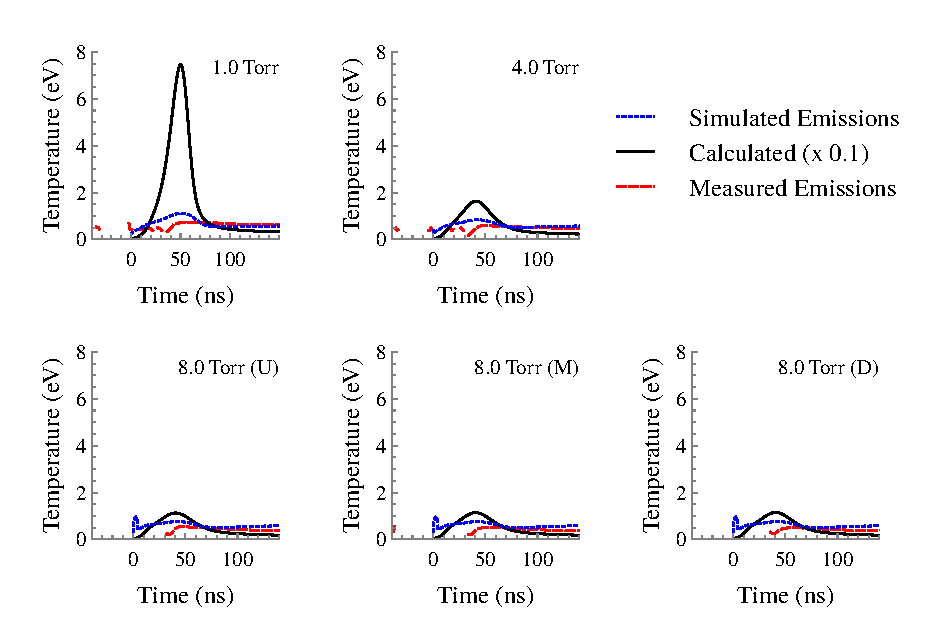
\includegraphics{./chapters/emissions/figures/boltcomp.eps}
  \caption{Temperatures estimated using Boltzmann plots of the measured emissions
    (dashed, red lines) and simulated emissions (dotted, blue lines) compared to
    the simulated temperatures (solid, black line).}
  \label{fig:boltcomp}
\end{figure}
The limited intensity of the plasma emissions prevented temperature estimates
for the experimental data soon after the pulse. Even after the emission
intensities rose to adequate values, the electron temperature estimates appeared
to be provide poor results for the duration of the measurement period. Peak
temperatures, relative to the actual results from the global model simulations,
were underestimated by at least a factor of ten, if not more.

This disagreement is not altogether unexpected. Even in the ideal case of
electron with a fixed temperature, \acs{plte} only occurs after each electron
has undergone many collisions with atoms in the gas. The changes in electron
temperatures of the \acs{rpnd} occur too rapidly for this kind of equilibrium to
occur. This is true, not only for the actual \acs{rpnd} operation, but the
simulation as well.

Based on this reasoning, it might be expected that the validity of the Boltzmann
plot approach would improve as the time increased. While this is eventually
true, it does not appear that the \acs{rpnd} afterglow ever reaches the point
where the all the states associated with the measured transitions reach
\acs{plte}. For the results shown, the Boltzmann plots for the measured and
simulated emissions continue to under-predict the electron temperatures well
into the afterglow. This reflects Kunze's statement that ``one always has to
check if indeed the assumption of a Boltzmann distribution is justified \ldots,
equilibrium may not be reached even if the steady-state conditions seem to
indicate that.'' \cite{Kunze2009}

Given this analysis, Boltzmann plots appear to be poor indicators of the
electron temperatures within an \acs{rpnd}. Though the results may improve as
the time after the pulse increases, it is possible that the emissions will fall
below detectable limits well before \acs{plte} applies. This is emphasized by an
examination of the individual Boltzmann plots, figure~\ref{fig:boltex},
\begin{figure}
  \centering
  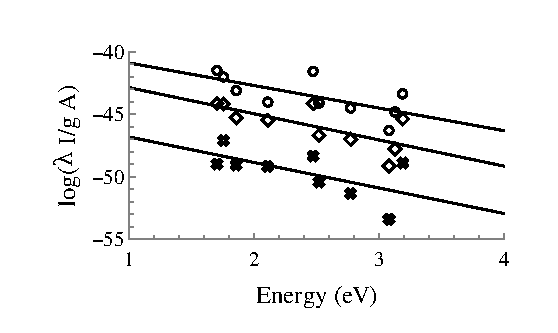
\includegraphics{./chapters/emissions/figures/boltex.eps}
  \caption{Boltzmann plot examples for the \acs{rpnd} at several different time
    points. Open symbols represent the measured values and the solid lines are
    the corresponding best fits.}
  \label{fig:boltex}
\end{figure}
obtained from the measurements. The open symbols represent the measurements for
three different times (circles - 50 ns after the pulse, diamonds - 1 $\mu$s,
crosses - 2 $\mu$s), and the straight lines are the best fits to the measured
data. While the trends are consistent between data sets, none appear to have the
linear trend which be expected for \acs{plte}, even several microseconds after
the pulse. Furthermore, while the electron temperatures should be different for
the wide range of times presented, the estimates only range from 0.5-0.55 eV.

\subsection{Coronal Model}

The failure of the \acs{plte} assumption indicates the need for a different
model in the determination of the electron temperature. One such model is the
coronal model. In this case, the excited states are all assumed to be generated
by electron collisions with ground state atoms. However, these excited states
decay by optical emission. This model excels at electron low densities where
states are not subject to a great degree of mixing and inter-atomic collisions
can be neglected \cite{Kunze2009}. As with \acs{plte}, it is not immediately
clear that these assumptions hold for the \acs{rpnd}.

Per Kunze \cite{Kunze2009}, the line intensity ratio resulting from the coronal
model may be expressed as
\begin{equation}
  \frac{I_{i,j}}{I_{i',j'}} = \frac{\lambda_{i',j'}A_{i,j}\sum A_{i'} K_{0,i}(T_e)}
  {\lambda_{i,j}A_{i',j'}\sum A_{i} K_{0,i'}(T_e)}
\end{equation}
where the sum is over all possible radiative decay pathways, the subscript `0'
is the ground state, and $K$ is the rate coefficient. Note that the rate
coefficients are explicitly functions of the electron temperature. As with the
global model, the rate coefficients must be calculated from the interaction
cross sections with an assumed \acs{eedf}. For consistency, we assume that this
is a Maxwell-Boltzmann distribution. The upper states used for this line ratio
must be carefully chosen so as to limit sensitivity to collisional mixing of
excited states. Likewise, the rate coefficient ratio should exhibit a monotonic
trend with electron temperature.

Kunze and others have suggested several line ratios for use with helium,
including: 4$^3$S-2$^3$P$\odd$ over 4$^1$S-2$^1$P$\odd$, 3$^3$S-2$^3$P$\odd$
over 3$^1$S-2$^1$P$\odd$, and 4$^3$S-2$^3$P$\odd$ over 4$^1$D-2$^1$P$\odd$. The
ratios with the upper state in an S subshell are attractive as they are less
have the lowest energy for a given $n$ and thus are less susceptible to
collisional mixing between states of equal $n$ \cite{Kunze2009}. However,
limited emission intensity prevented accurate measurements of the
4$^1$S-2$^1$P$\odd$ transition. As a result, only the former two ratios were
considered for analysis.

Like the other mentioned ratios, 4$^3$S-2$^3$P$\odd$ over 4$^1$D-2$^1$P$\odd$
compares a transition from the triplet manifold to one from the singlet
manifold. Triplet-singlet ratios have been found to be mostly dependent to
electron temperature which makes them ideal for this purpose \cite{Griem2005}.
Figure~\ref{fig:conversion}
\begin{figure}
  \centering
  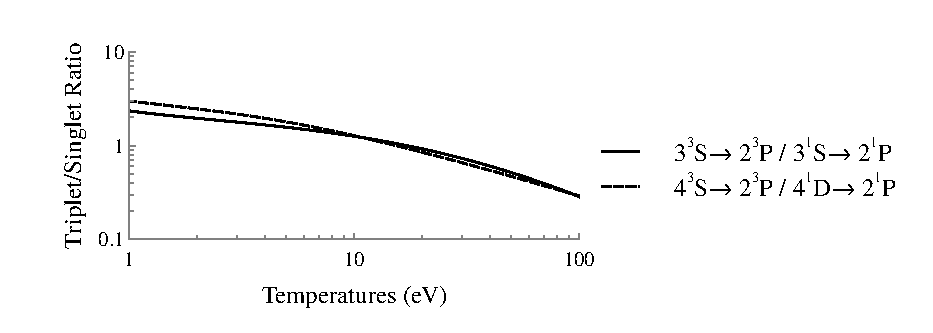
\includegraphics{./chapters/emissions/figures/conversion.eps}
  \caption{The emission ratios of 4$^3$S-2$^3$P$\odd$ over 4$^1$D-2$^1$P$\odd$ 
    and 3$^3$S-2$^3$P$\odd$ over 3$^1$S-2$^1$P$\odd$, as functions of the
    electron temperature.}
  \label{fig:conversion}
\end{figure}
shows the relation between the emission intensity of the two transitions and the
electron temperature of the system. The rate coefficients were calculated with
the assumption of a Maxwell-Boltzmann distribution, using the cross sections
produced by Ralchenko et al. \cite{Ralchenko2008}. 

These calculations for the triplet-singlet ratios were used to estimate the
electron temperature from the simulated emissions as well as the measured
emissions. As with the Boltzmann plots, the temperatures calculated from the
simulated emissions represent the best attainable result with this method. The
results obtained with the 4$^3$S-2$^3$P$\odd$ to 4$^1$D-2$^1$P$\odd$ ratio, seen
in figure~\ref{fig:rat2comp},
\begin{figure}
  \centering
  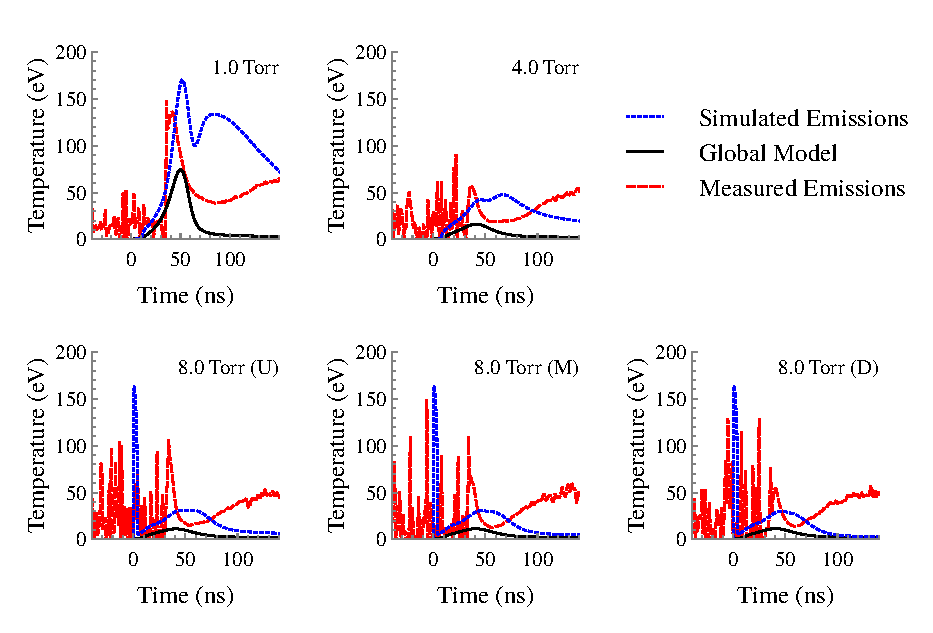
\includegraphics{./chapters/emissions/figures/rat2comp.eps}
  \caption{Estimates of the electron temperatures based on the ratio of the
    4$^3$S-2$^3$P$\odd$ and 4$^1$D-2$^1$P$\odd$ transitions. The estimates were
    generated for the simulated emissions (dotted, blue lines) and measured
    emissions (dashed, red lines), and are compared to the actual temperature
    results from the global model simulation (solid, black lines).}
  \label{fig:rat2comp}
\end{figure}
were not promising. As before, neither the simulated nor the measured ratios
proved to provide good estimates of the electron temperatures. However, unlike
the Boltzmann plots, this line ratio generally resulted in an overestimate of
the temperatures. The signal prior to 30 ns is marked by a large amount of
spurious results. This is attributable to the very small optical signals during
this time period. After 30 ns, once the emission intensities have reached
relatively large values, the large variations in the temperature estimates
disappear.

Based on the curve for this ratio from figure~\ref{fig:conversion}, the high
temperature estimates indicate a low value for the triplet-singlet ratio. This
suggests either an excess in 4$^1$D states, or a deficit of 4$^3$S states.
Additionally, both the measured and simulated ratios show growing or otherwise
elevated temperature well after the pulse. This may be partially explained by
the use of the 4$^1$D state for the singlet transition, an approach warned
against by Kunze \cite{Kunze2009}.

Also notable is the disagreement between the measured and simulated ratios.
While the temperatures estimated from the measurements quickly decrease after
the pulse, the temperatures from the simulations continue to rise. This
situation reverses at about 75 ns when the temperature estimates from the
measurements begin to rise while the simulated ones fall. The reason for this
difference in behavior is not immediately clear, however Boivin et al.\ reported
several problems with this line ratio which they attributed to the omission of
$n=5$ states from their simulations \cite{Boivin2007}. 

Unlike the prior line ratio, a comparison of 3$^3$S-2$^3$P$\odd$ to
3$^1$S-2$^1$P$\odd$, removes the use of a D subshell for the upper level.
Therefore this set of transitions should be less susceptible to collisional
effects. Additionally, the lower $n$ results in a greater energy spacing between
the different subshells. For both of these reasons, this ratio should be less
susceptible to collisional mixing. While the lower threshold energies make this
ratio less desirable for very high electron temperatures, it was believed to be
more than adequate for the \acs{rpnd}. This reasoning is somewhat borne out by
the results in figure~\ref{fig:rat1comp}.
\begin{figure}
  \centering
  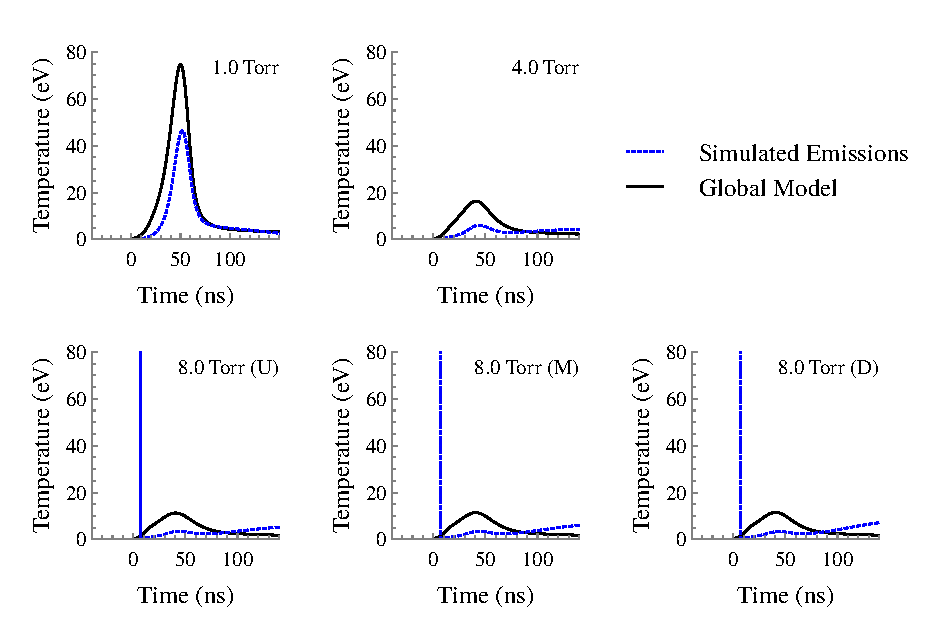
\includegraphics{./chapters/emissions/figures/rat1comp.eps}
  \caption{Estimates of the electron temperatures based on the ratio of the
    3$^3$S-2$^3$P$\odd$ to 3$^1$S-2$^1$P$\odd$, transitions. The estimates were
    generated for the simulated emissions (dotted, blue lines) and measured
    emissions (dashed, red lines), and are compared to the actual temperature
    results from the global model simulation (solid, black lines).}
  \label{fig:rat1comp}
\end{figure}

The temperature estimates based on the simulated emissions show excellent
agreement with the temperatures from the global model. This does not confirm the
temperature predictions made by the global model, however it does demonstrate
the promise of this approach compared to the previous line ratio. The simulated
emission results match both the magnitude of the values and the overall behavior
of the trends. The initial increase in temperature is captured particularly
well, with only moderate deviations in the afterglow. These differences are
believe to be the result of the radiative cascade from higher excited states
which contribute to the population of the upper excited states, mildly violating
the coronal model.

Unfortunately, the experimental results do not appear to bear out the promise
indicated by the simulated emissions. From a fundamental perspective, this
temperature estimate is based on predictions which assume a Maxwell-Boltzmann
distribution, an assumption which may not be valid for the \acs{rpnd}. That
said, while the results from figure~\ref{fig:rat1comp} may not correspond to an
equilibrium \acs{eedf}, they can provide a relative comparison of mean electron
energies.

Aside from the possible complications introduced by the distribution
assumptions, estimates using this line ratio were also impacted by experimental
difficulties. The two transitions occur at wavelengths to which the \acs{pmt} is
noticeably less sensitive. As a result, the absolute intensities of these lines
were particularly low. This led to substantial uncertainties in the line
ratios, particularly for times prior to 30 ns and, to some extent, afterward.

Of the available data, the two transitions were most intense at 4.0 Torr. As a
result, this represents the most accurate measurements of the line ratio in
described cases. In contrast to the temperatures produced by the global model,
the 4.0 Torr emission measurements suggest that the temperature peaks at 4.9 eV
followed by a rapid relaxation to about 0.5 eV. If accurate, the fast relaxation
of the electrons suggests that additional inelastic processes should be
considered by the global model. The most likely reservoir for this energy would
be the excited states of molecular nitrogen which is believed to compose about
70\% of the estimated 80 ppm of impurities in the system.

Given the low intensities, difficulty in obtaining accurate intensity
measurements \cite{Griem2005}, and the sensitivity of the temperature estimate
to the line ratio, these results should be considered quite preliminary. The use
of these transitions is promising for measurements of the electron temperature
in the \acs{rpnd}--the global model simulations show a good agreement between
the estimates and the actual temperatures, and the ratio changes quickly enough
to capture at least some of the \acs{rpnd} dynamics. That said, the use of a
Maxwell-Boltzmann distribution in the line ratio calculations may need to be
reconsidered. Additionally, improvements to the spectral sensitivity at these
wavelengths are necessary in order to confirm the presented measurements and to
better understand the discrepancies with the simulation.

\section{Emission Comparisons}

The emission curves of the simulated and experimental \acs{rpnd} contain a
number of minor and significant differences. Likewise, some provide meaningful
insight on the plasma characteristics, others are more ambiguous. For example,
the greater than expected prominence of the 4$^3$D-2$^3$P$\odd$ transition at
447 nm may either indicate a more substantial high energy electron tail, or the
need for the inclusion of $n=5$ states. Two differences will be analyzed here,
however the full set of emission measurements are presented in
Appendix~\ref{chp:extraem}.

\subsection{Excitation Duration}

As was noted in Chapter~\ref{chp:modeling}, several assumptions were needed to
develop the global model used to simulate the \acs{rpnd}. Among these were the
assumption that the \acs{eedf} was always a Maxwell-Boltzmann distribution, and
that the applied electric field was a Gaussian function in time with a width of
40 ns. The \acs{pic} simulations as well as the results from Boltzmann plots and
line ratios have already suggested that the former assumption is not rigorously
true. While the electric field shape was originally inferred from the
observation of a return stroke in the system, this assumption was considered in
more detail via the 3$^1$D-2$^1$P$\odd$ transition at 668 nm.

Figure~\ref{fig:dpcomp}
\begin{figure}
  \centering
  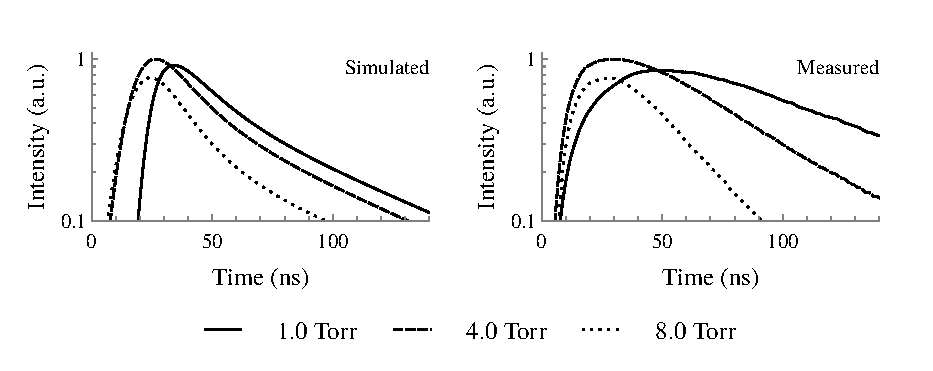
\includegraphics{./chapters/emissions/figures/dpcomp.eps}
  \caption{Comparison of the measured and simulated emissions from the
  3$^1$D-2$^1$P$\odd$ transition at pressures of 1.0, 4.0, and 8.0 Torr.}
  \label{fig:dpcomp}
\end{figure}
features a comparison of the measured and simulated emissions for the
3$^1$D-2$^1$P$\odd$ transition over the range of simulated pressures. Both sets
of results have been normalized to the maximum value of the 4.0 Torr transition
so that the relative trends could be compared. 

This transition was initially chosen for investigation because it was
particularly prominent in both the measured and simulated emissions.
Additionally, at $n=3$, the upper state is below the maximum $n$ considered in
the global model. Therefore, the evolution of the upper state density and its
emission curve reflects re-population effects as a result of radiative decay
from $n=4$. Finally, the comparative behavior of the emission curves is
representative of most of the other transitions.

The simulations and the experimental measurements share a number general
features. The optical intensity peaks at 4.0 Torr, followed by 1.0 Torr, and
lastly, by 8.0 Torr. The relative magnitude of the optical intensities also
agree for times greater than 50 ns after the pulse. Additionally, the timing of
the peaks are also consistent between the two sets of data. It is interesting to
note that this occurs in part because of the long delay before the onset of the
emissions in the 1.0 Torr simulation.

Despite the similarities, there are several notable differences. As already
mentioned, there is a significant delay prior to the appearance of emissions
from the 1.0 Torr simulation. This is probably caused by the low pre-pulse
electron density in the 1.0 Torr case--approximately two orders of magnitude
less than the other cases. Though this value is believed to be accurate, this
behavior must be reconciled with that of the observed emissions which all appear
at approximately the same time.

Also observable is an apparent pressure dependence for the rate at which the
measured emissions grew. At 1.0 Torr, the emissions took noticeably longer to
reach their peak intensity as compared to the measurements at 8.0 Torr, or 4.0
Torr which was the fastest. This is similar to what appeared to be a relatively
slow growth in the metastable density at 1.0 Torr, as seen in
figure~\ref{fig:nmcomp}. Again, this suggests that something unexpected is
occurring at the 1.0 Torr condition. To some extent, the behavior of the
emissions and the metastable densities almost appear to be the result of a
broadening of the applied voltage pulse.

It may also be explained by a more beam-like \acs{eedf} with an elevated
population of high-energy electrons. Interaction cross sections monotonically
decline for electrons with energies greater than about 10 eV. This extends the
time required for the high energy electrons to interact with the surrounding
gas. Similarly broad emission curves were observed in the 0.5 and 0.3 Torr
experiments as well.

Another important difference is the post-pulse shape of the curves. The
simulated emissions, after reaching their peak, have decays which could be best
described by a superposition of a fast and a slow component. This behavior--a
fast decay following the pulse followed by a slow one, is similar to the
behavior of the electron temperature from figure~\ref{fig:etemps}. It seems
likely that the two are related as the fast fall in electron temperature would
result in a fall of the excitation rate of the 3$^1$D state, reducing its
emissions.

By comparison, each of the measured emission curves are best matched by a single
exponential decay process. While the slow exponential decay rate of the
simulated results is relatively constant across pressures, there is a distinct
pressure dependence in the measured emissions. This tends to suggest some type
of atomic collision process as the global model provides a relatively complete
accounting for the electron collision processes. Likewise, excitation transfer
processes were also considered. The next most likely candidate would by the
impurities within the system which were not included in the model. 

\section{Summary}

The active spectroscopy used to measure the metastable densities within the
\acs{rpnd} and the subsequent modeling provided a number of insights on its
development. Passive spectroscopy was then used to provide further information
on the development of the discharge. Initial analysis of the emissions indicated
that the wave developed with a velocity of 1.7-3.0$\times10^7$ m/s at 8.0 Torr
and 0.7-1.5$\times10^7$ m/s at 16.0 Torr. All other operating conditions
developed with velocities in excess of 5.0$\times10^7$ m/s.

Estimates of the wave velocity were followed by several attempts to determine
the evolution of the electron temperature in the \acs{rpnd}. This included the
use of Boltzmann plots (with the corresponding assumption of \acs{plte}), as
well as line ratios based on the coronal excitation model. The Boltzmann plot
method proved to be a poor and unreliable indicator of electron temperature in
the system. Examination of the individual Boltzmann plots revealed that the
excited states were far from \acs{plte}. Attempts to use the ratio of the
4$^3$S-2$^3$P$\odd$ to the 4$^1$D-2$^1$P$\odd$ transition also proved to be
fruitless as even the temperatures from the simulated emissions did not match
the actual temperatures in the gloval model. Eventually the simulated emission
ratio of 3$^3$S-2$^3$P$\odd$ over 3$^1$S-2$^1$P$\odd$, was shown to provide good
agreement with the temperatures of the global model. However, use of this line
ratio with the actual \acs{rpnd} was limited by experimental uncertainties.

The emissions of the \acs{rpnd} were further analyzed for three transitions. The
measured and simulated 3$^1$D-2$^1$P$\odd$ emissions were considered because of
their prominence and representative nature. General trends such as the relative
emission intensities and timing of the peak intensities were consistent between
the simulations and measurements. However, several significant differences also
appeared. The decay of the experimental emissions featured a notable pressure
dependence which was not present in the simulated emissions. It was speculated
that this resulted from collisional processes with impurities which were not
accounted for in the global model. Additionally, the 1.0 Torr measurements
showed an unusually extended excitation period. This trend continued to the
lower pressures, and the metastable trends at 1.0 Torr appear to support the
existence of an extended excitation period. The reason for this change in
behavior at low pressures is not entirely clear though it was speculated to be
the result of an excess in high energy electrons.
